\RCS$Revision: 342265 $
\RCS$HeadURL: svn+ssh://bainbrid@svn.cern.ch/reps/tdr2/papers/SUS-14-006/trunk/SUS-14-006.tex $
\RCS$Id: SUS-14-006.tex 342265 2016-05-10 19:38:31Z bainbrid $

\newlength\cmsFigWidth
\ifthenelse{\boolean{cms@external}}{\setlength\cmsFigWidth{0.85\columnwidth}}{\setlength\cmsFigWidth{0.4\textwidth}}
\ifthenelse{\boolean{cms@external}}{\providecommand{\cmsLeft}{top}}{\providecommand{\cmsLeft}{left}}
\ifthenelse{\boolean{cms@external}}{\providecommand{\cmsRight}{bottom}}{\providecommand{\cmsRight}{right}}

\newcommand{\kfactor}{\ensuremath{k\text{-factor}}\xspace}
\newcommand{\kfactors}{\ensuremath{k\text{-factors}}\xspace}
\newcommand{\njet}{\ensuremath{n_{\text{jet}}}\xspace}
\newcommand{\njetlow}{\ensuremath{2 \leq \njet \leq 3}\xspace}
\newcommand{\njethigh}{\ensuremath{\njet \geq 4}\xspace}
\newcommand{\nb}{\ensuremath{n_{\text{b}}}\xspace}
\newcommand{\alphat}{\ensuremath{\alpha_{\text{T}}}\xspace}
\newcommand{\alphatcut}{\ensuremath{\alpha_{\text{T}}^{\text{cut}}}\xspace}
\newcommand{\htalphat}{\texttt{HT\_AlphaT}\xspace}
\newcommand{\photon}{\texttt{Photon}\xspace}
\newcommand{\muht}{\texttt{Mu\_HT}\xspace}
\newcommand{\httrigger}{\texttt{HT}\xspace}
\newcommand{\mt}{\ensuremath{M_{\textrm T}}\xspace}
\newcommand{\gj}{\ensuremath{\gamma} + jets\xspace}
\newcommand{\mj}{\ensuremath{\mu} + jets\xspace}
\newcommand{\mmj}{\ensuremath{\mu\mu} + jets\xspace}
\newcommand{\npre}{\ensuremath{N_{\textrm{pred}}}\xspace}
\newcommand{\nobs}{\ensuremath{N_{\textrm{obs}}}\xspace}
\newcommand{\njets}{\ensuremath{N_{\textrm{jet}}}\xspace}
\newcommand{\sq}{\ensuremath{\tilde{\rm q}}\xspace}
\newcommand{\st}{\ensuremath{\tilde{\rm t}}\xspace}
\newcommand{\gl}{\ensuremath{\tilde{\rm g}}\xspace}
\newcommand{\dht}{\ensuremath{\Delta\scalht}\xspace}
\newcommand{\ewk}{\ensuremath{\mathrm{EWK}}\xspace}
\newcommand{\qcd}{\ensuremath{\mathrm{QCD}}\xspace}
\newcommand{\fZinv}[1]{\ensuremath{f_{\rm Zinv}^{#1}}\xspace}
\newcommand{\zInv}[1]{\ensuremath{Z_{\rm inv}^{#1}}\xspace}
\newcommand{\meanHt}[1]{\ensuremath{\langle \HT \rangle^{#1}}\xspace}
\newcommand{\lk}[2]{\ensuremath{L^{\rm #1}_{\rm #2}}\xspace}
\newcommand{\sep}{\ensuremath{68^{\mathrm{th}}}\xspace}
\newcommand{\partonht}{\ensuremath{\scalht^{\rm parton}}\xspace}
\newcommand{\meff}{\ensuremath{M_{\rm eff}}\xspace}
\newcommand{\mhttt}{\ensuremath{\hslash_{\rm T}^{TT}}\xspace}



\cmsNoteHeader{SUS-14-006} 

\title{Search for top squark pair production in
  compressed-mass-spectrum scenarios in proton-proton collisions at
  $\sqrt{s} = 8\TeV$ using the \alphat variable}

\date{\today}

\abstract{This document contains the supplementary material to support
the publication.}
%\abstract{An inclusive search is performed for supersymmetry in final
%  states containing jets and an apparent imbalance in transverse
%  momentum, \ptvecmiss, due to the production of unobserved weakly
%  interacting particles in pp collisions at a centre-of-mass energy of
%  8\TeV. The data, recorded with the CMS detector at the CERN LHC,
%  correspond to an integrated luminosity of 18.5\fbinv. The
%  dimensionless kinematic variable \alphat is used to discriminate
%  between events with genuine \ptvecmiss associated with unobserved
%  particles and spurious values of \ptvecmiss arising from jet energy
%  mismeasurements. No excess of event yields above the expected
%  standard model backgrounds is observed. The results are interpreted
%  in terms of constraints on the parameter space of several simplified
%  models of supersymmetry that assume the pair production of top
%  squarks. The search provides sensitivity to a broad range of top
%  squark ($\sTop$) decay modes, including the two-body decay $\sTop
%  \!\rightarrow\!  \text{c} \chiz_1$, where c is a charm quark and
%  $\chiz_1$ is the lightest neutralino, as well as the four-body decay
%  $\sTop \!\rightarrow\!  {\rm b f \bar{f^{'}}} \chiz_1$, where b is a
%  bottom quark and f and ${\rm \bar{f^{'}}}$ are fermions produced in
%  the decay of an intermediate off-shell W boson. These modes dominate
%  in scenarios in which the top squark and lightest neutralino are
%  nearly degenerate in mass. For these modes, top squarks with masses
%  as large as 260 and 230\GeV are excluded, respectively, for the two-
%  and four-body decays.}

\hypersetup{
pdfauthor={M. Baber, R. Bainbridge, O. Buchmueller, D. Burton, M. Citron, A. Elwood, Y. Eshaq, H. Flaecher, A. Garcia-Bellido, E. Laird, K. Lo, C. Lucas, J. Marrouche, Z. Meng, T. Sakuma, D. Smith, and A. Tapper},
pdftitle={Search for top squark pair production in compressed-mass-spectrum scenarios in proton-proton collisions at sqrt(s) = 8 TeV using the alphaT variable},
pdfsubject={CMS},
pdfkeywords={CMS, physics, SUSY, jets, missing transverse momentum, alphaT}
}

\maketitle

%%%%%%%%%%%%%%%%%%%%%%%%%%%%%%%%%%%%%%%%%%%%%%%%%%%%%%%%%%%%%%%%%%%%%%%%%%%%%%%%

\clearpage
\begin{figure*}[h!]
  \begin{center}
    \includegraphics[width=0.49\textwidth,page=2]{figures/fit_result/bestFit_2012dev_RQcdZero_fZinvAll_0b_le3j-12p_smOnly} 
    \includegraphics[width=0.49\textwidth,page=2]{figures/fit_result/bestFit_2012dev_RQcdZero_fZinvAll_0b_le3j-12hp_smOnly} \\
    \caption{\label{fig:best-fit-0b} Candidate signal event yields
      observed in data (solid circles) and SM expectations with their
      associated uncertainties (solid lines with bands) in bins of
      \scalht for events that satisfy \njetlow and $\nb = 0$. (Left)
      SM a priori expectations. (Right) SM expectations from the fit
      including the signal region. }
  \end{center}
\end{figure*}

\begin{figure*}[h!]
  \begin{center}
    \includegraphics[width=0.49\textwidth,page=2]{figures/fit_result/bestFit_2012dev_RQcdZero_fZinvAll_0b_ge4j-12p_smOnly} 
    \includegraphics[width=0.49\textwidth,page=2]{figures/fit_result/bestFit_2012dev_RQcdZero_fZinvAll_0b_ge4j-12hp_smOnly} \\
    \caption{\label{fig:best-fit-0b} Candidate signal event yields
      observed in data (solid circles) and SM expectations with their
      associated uncertainties (solid lines with bands) in bins of
      \scalht for events that satisfy \njethigh and $\nb = 0$. (Left)
      SM a priori expectations. (Right) SM expectations from the fit
      including the signal region. }
  \end{center}
\end{figure*}

\clearpage
\begin{figure*}[h!]
  \begin{center}
    \includegraphics[width=0.49\textwidth,page=2]{figures/fit_result/bestFit_2012dev_RQcdZero_fZinvAll_1b_le3j-12p_smOnly} 
    \includegraphics[width=0.49\textwidth,page=2]{figures/fit_result/bestFit_2012dev_RQcdZero_fZinvAll_1b_le3j-12hp_smOnly} \\
    \caption{\label{fig:best-fit-0b} Candidate signal event yields
      observed in data (solid circles) and SM expectations with their
      associated uncertainties (solid lines with bands) in bins of
      \scalht for events that satisfy \njetlow and $\nb = 1$. (Left)
      SM a priori expectations. (Right) SM expectations from the fit
      including the signal region. }
  \end{center}
\end{figure*}

\begin{figure*}[h!]
  \begin{center}
    \includegraphics[width=0.49\textwidth,page=2]{figures/fit_result/bestFit_2012dev_RQcdZero_fZinvAll_1b_ge4j-12p_smOnly} 
    \includegraphics[width=0.49\textwidth,page=2]{figures/fit_result/bestFit_2012dev_RQcdZero_fZinvAll_1b_ge4j-12hp_smOnly} \\
    \caption{\label{fig:best-fit-0b} Candidate signal event yields
      observed in data (solid circles) and SM expectations with their
      associated uncertainties (solid lines with bands) in bins of
      \scalht for events that satisfy \njethigh and $\nb = 1$. (Left)
      SM a priori expectations. (Right) SM expectations from the fit
      including the signal region. }
  \end{center}
\end{figure*}

\clearpage
\begin{figure*}[h!]
  \begin{center}
    \includegraphics[width=0.49\textwidth,page=2]{figures/fit_result/bestFit_2012dev_RQcdZero_fZinvAll_2b_le3j-1_smOnly} 
    \includegraphics[width=0.49\textwidth,page=2]{figures/fit_result/bestFit_2012dev_RQcdZero_fZinvAll_2b_le3j-1h_smOnly} \\
    \caption{\label{fig:best-fit-0b} Candidate signal event yields
      observed in data (solid circles) and SM expectations with their
      associated uncertainties (solid lines with bands) in bins of
      \scalht for events that satisfy \njetlow and $\nb = 2$. (Left)
      SM a priori expectations. (Right) SM expectations from the fit
      including the signal region. }
  \end{center}
\end{figure*}

\begin{figure*}[h!]
  \begin{center}
    \includegraphics[width=0.49\textwidth,page=2]{figures/fit_result/bestFit_2012dev_RQcdZero_fZinvAll_2b_ge4j-1_smOnly} 
    \includegraphics[width=0.49\textwidth,page=2]{figures/fit_result/bestFit_2012dev_RQcdZero_fZinvAll_2b_ge4j-1h_smOnly} \\
    \caption{\label{fig:best-fit-0b} Candidate signal event yields
      observed in data (solid circles) and SM expectations with their
      associated uncertainties (solid lines with bands) in bins of
      \scalht for events that satisfy \njethigh and $\nb = 2$. (Left)
      SM a priori expectations. (Right) SM expectations from the fit
      including the signal region. }
  \end{center}
\end{figure*}

\clearpage
\begin{figure*}[h!]
  \begin{center}
    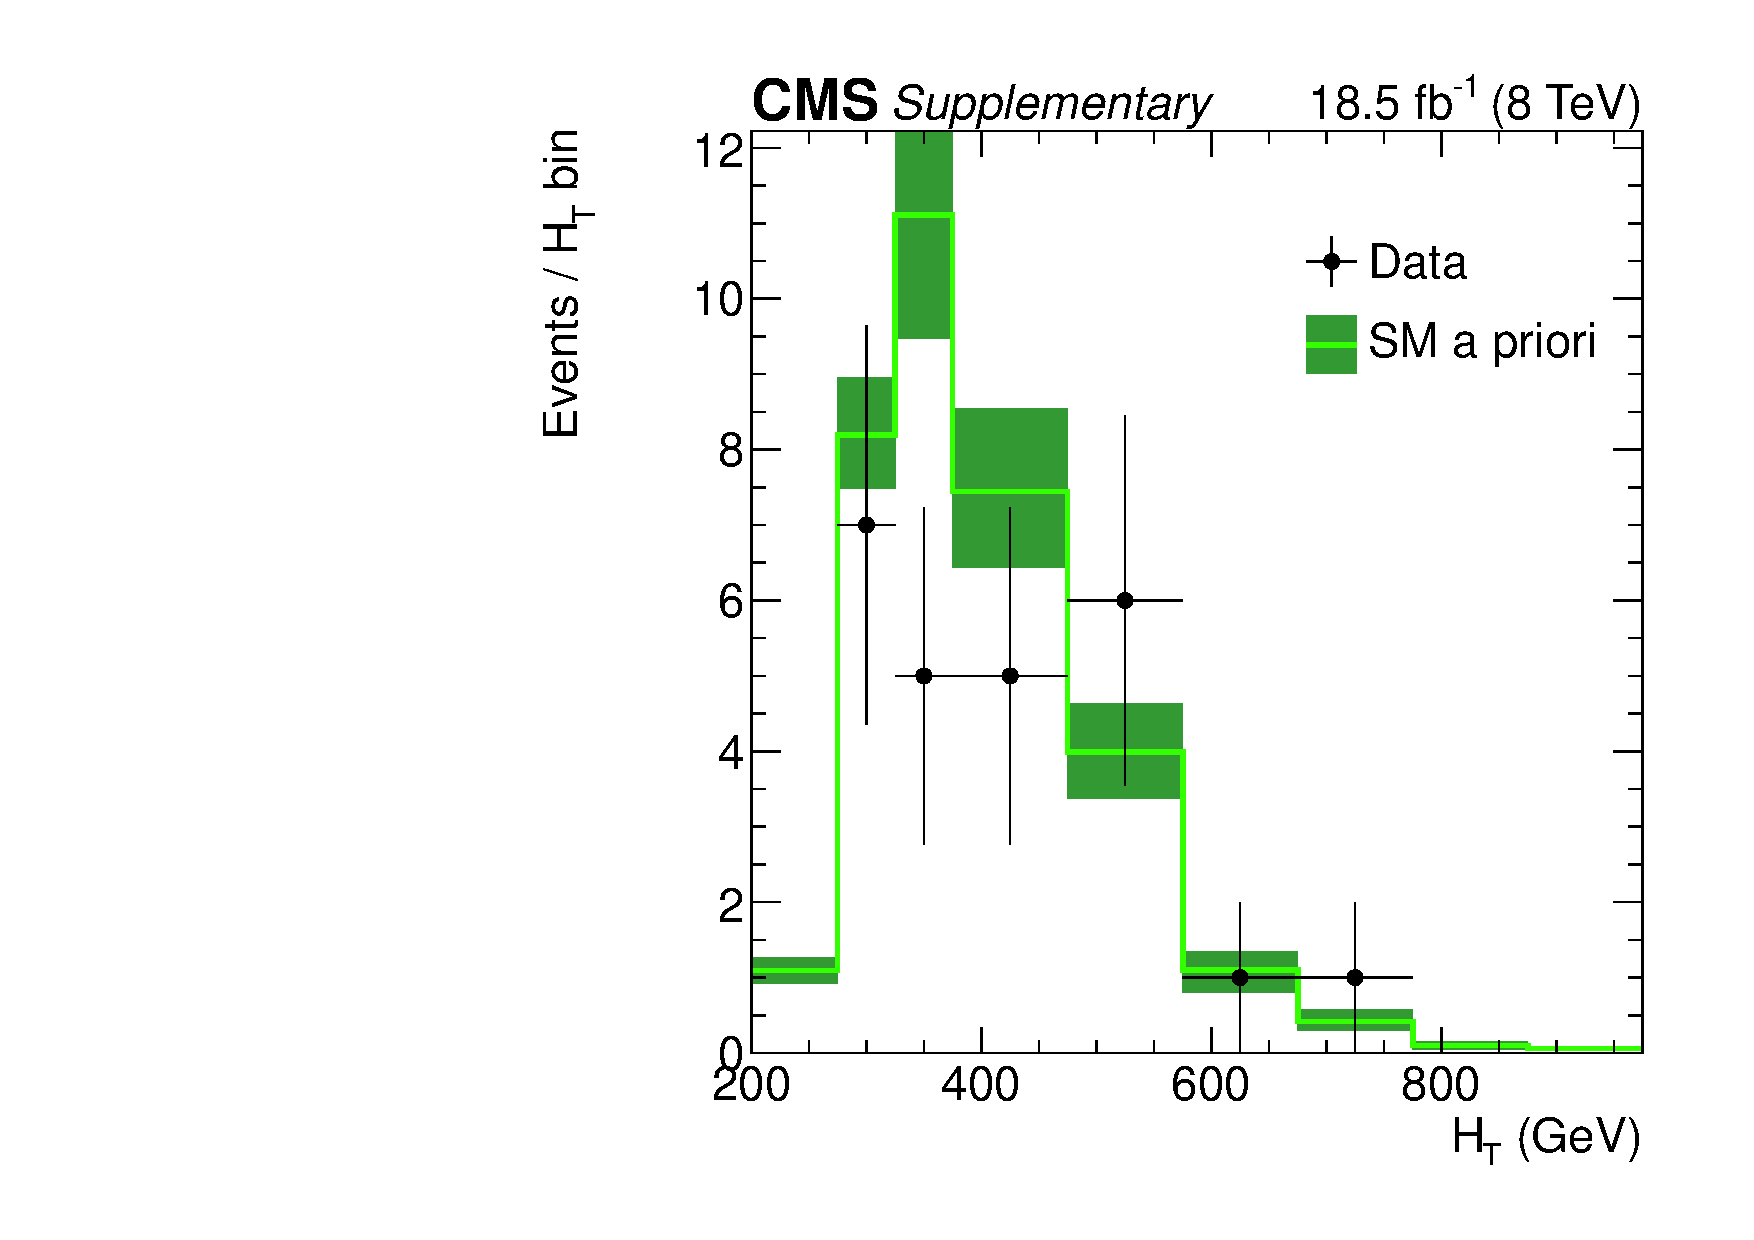
\includegraphics[width=0.49\textwidth,page=1]{figures/fit_result/bestFit_2012dev_RQcdZero_fZinvAll_3b_ge4j-1_smOnly} 
    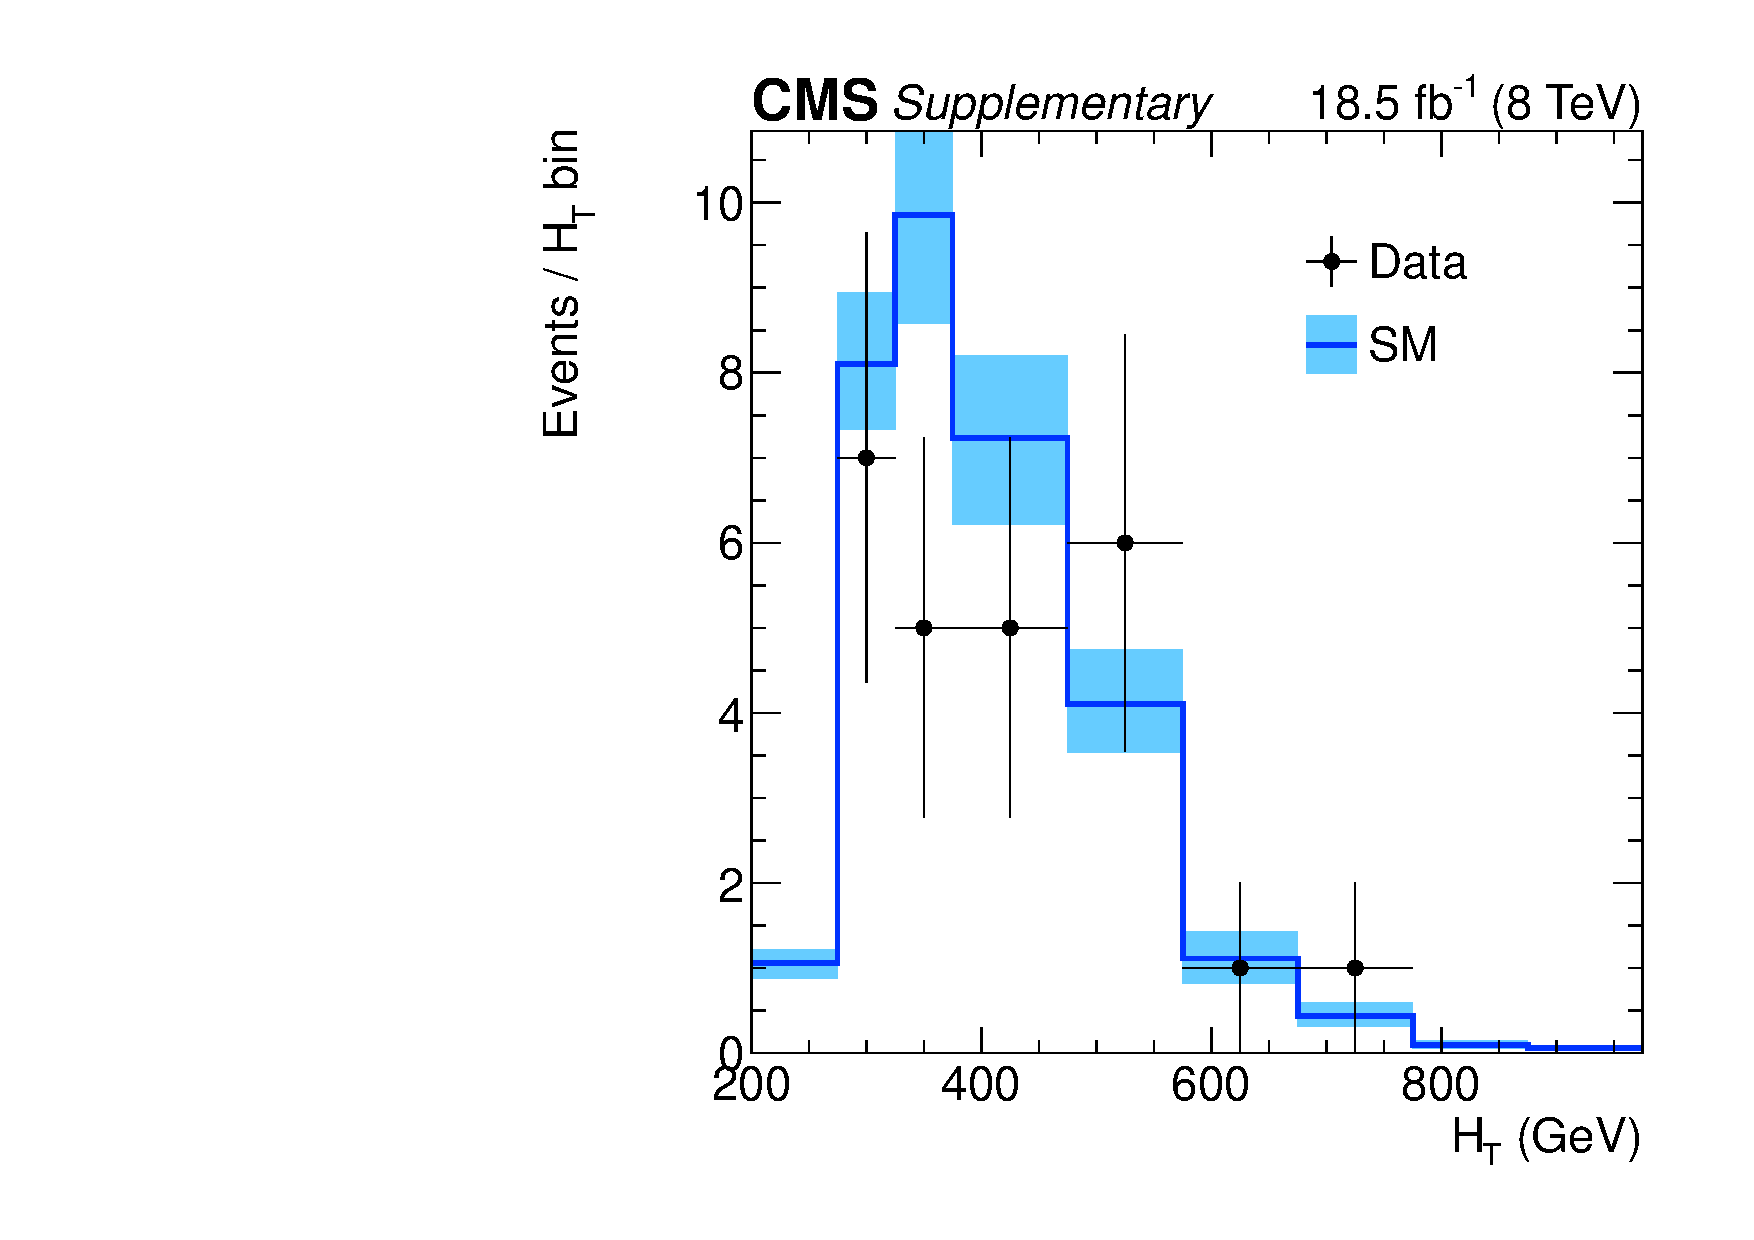
\includegraphics[width=0.49\textwidth,page=1]{figures/fit_result/bestFit_2012dev_RQcdZero_fZinvAll_3b_ge4j-1h_smOnly} \\
    \caption{\label{fig:best-fit-0b} Candidate signal event yields
      observed in data (solid circles) and SM expectations with their
      associated uncertainties (solid lines with bands) in bins of
      \scalht for events that satisfy \njethigh and $\nb = 3$. (Left)
      SM a priori expectations. (Right) SM expectations from the fit
      including the signal region. }
  \end{center}
\end{figure*}

\begin{figure*}[h!]
  \begin{center}
    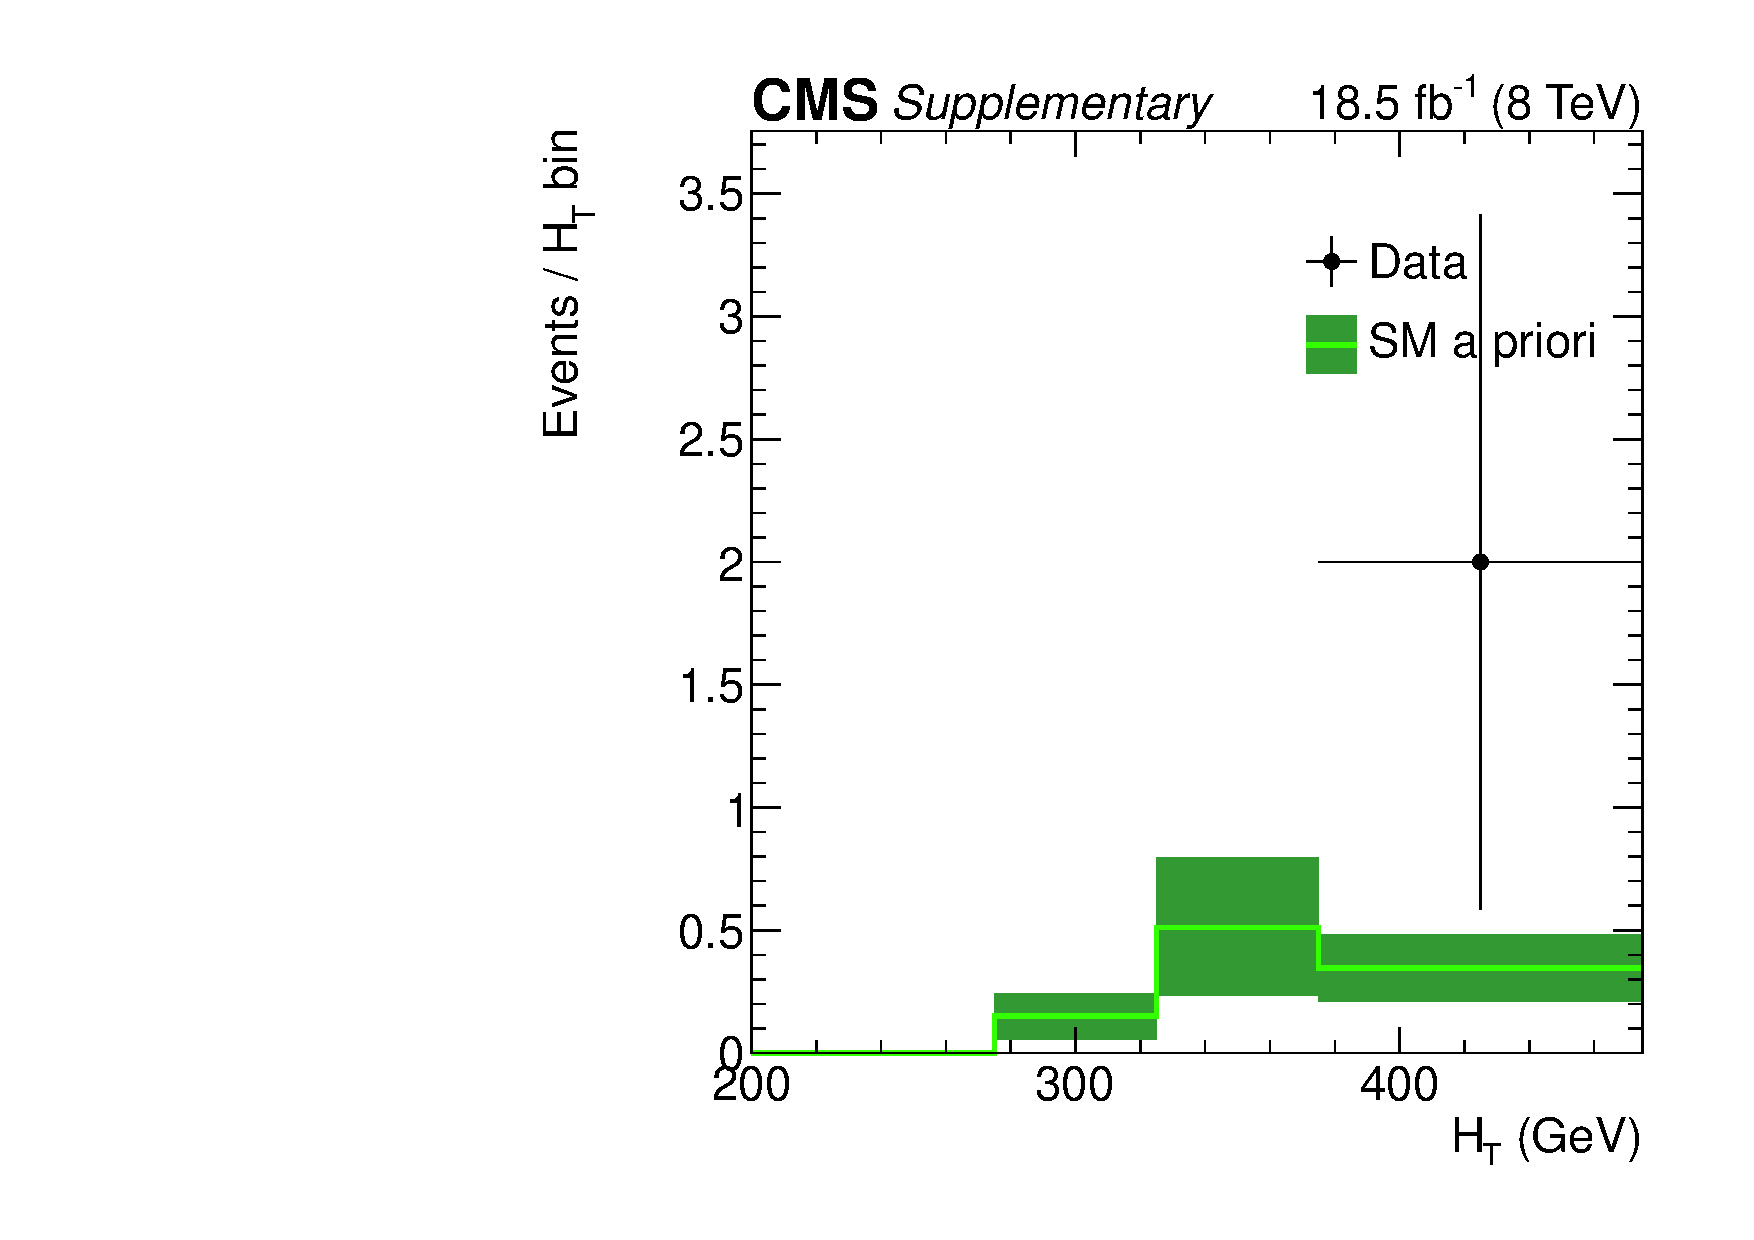
\includegraphics[width=0.49\textwidth,page=1]{figures/fit_result/bestFit_2012dev_RQcdZero_fZinvAll_ge4b_ge4j-1_smOnly} 
    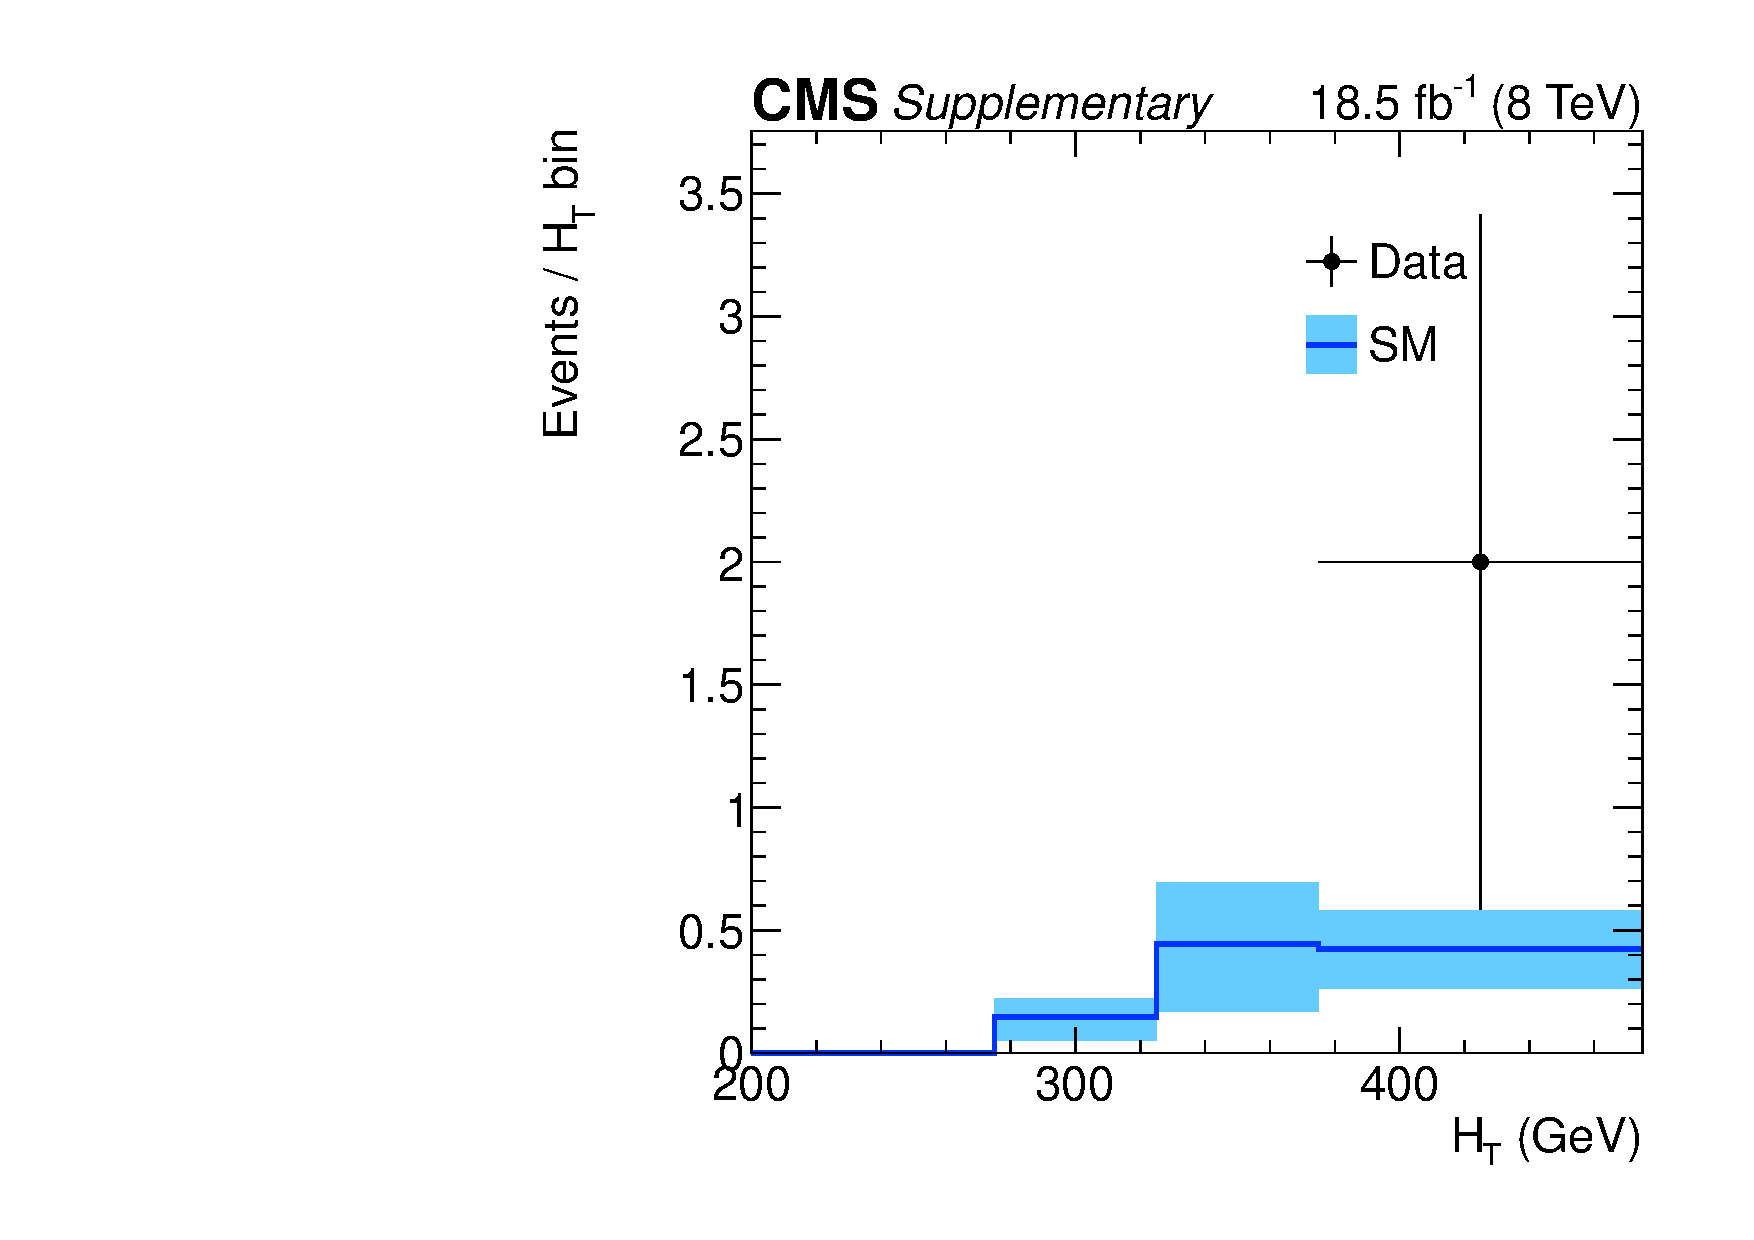
\includegraphics[width=0.49\textwidth,page=1]{figures/fit_result/bestFit_2012dev_RQcdZero_fZinvAll_ge4b_ge4j-1h_smOnly} \\
    \caption{\label{fig:best-fit-0b} Candidate signal event yields
      observed in data (solid circles) and SM expectations with their
      associated uncertainties (solid lines with bands) in bins of
      \scalht for events that satisfy \njethigh and $\nb \geq
      4$. (Left) SM a priori expectations. (Right) SM expectations
      from the fit including the signal region. }
  \end{center}
\end{figure*}

%%%%%%%%%%%%%%%%%%%%%%%%%%%%%%%%%%%%%%%%%%%%%%%%%%%%%%%%%%%%%%%%%%%%%%%%%%%%%%%%

%\clearpage
%\bibliography{auto_generated}
